\begin{comment}

Key ideas:

- Pictures
- Requirements
    - Can split relatively positioned elements
    - Relative and changing (increasing, decreasing) size 
    - Repetitive
    - Human understandable
    - Linked, indexed, sorted, consecutive



% Major problem with such geometric data, is that similar elements from different drawings are relatively positioned and scaled. To illustrate such state, I combined multiple Luria 'P' tests from different individuals on single Figure \ref{luria-multiple} with original \textit{x, y} coordinates. 

% If we take a look at single Luria's 'P' line on Figure \ref{luria-single}, we should notice, that pattern consists of connected repetitive horizontal and vertical lines.

% & Algorithm should handle repetitive elements
% & Similar elements from different drawings may have relative position, size and scale
% & Elements may vary in position and size within single pattern
% & Clusters should be interpretable
% & Clusters should be ordered




% \begin{easylist}

% & Should encapsulate logic and data of a cluster
% & Should contain

% \end{easylist}

% \subsection{Edge Entity Generation}

% \begin{easylist}

% & Pairs of corner neighbour nodes determined, N consecutive corner nodes yield N-1 pairs

% & N-1 Edges generated from N-1 pairs of corner nodes and saved in corresponding list $edges_depth_0_list$ 

% & For each Edge in the edges_depth_0_list M Sub-Edges are created and saved in another list edges_depth_1_list

% \end{easylist}


% After completion of previous phase, \textit{Drawing} entity is complemented with ordered list of corners nodes (Figure \ref{clustering-1}). List of corner nodes are sorted by node timestamp \textit{t} in descending order. Each pair of consecutive neighbour nodes represent a meaningful cluster of a pattern or \textit{Edge} entity. \textit{Edge} entity encapsulates meta-information and data points of certain segment of the Drawing. 

% Consecutive neighbour corner node pairs produce \textit{n} Edge entities. Therefore, clustering of Luria 'PL' pattern should yield \textit{n = 28} edges.
% To improve precision, it is possible to split each Edge recursively into \textit{m} Sub-Edges. By intuition, edge is a stroke of the drawing and each stroke may have \textit{[starting, ending] }or \textit{[starting, middle, ending]} parts, therefore we can split Edge into $m = 2$ or $m = 3$ logical parts.

% Process can be repeated recursively required number of times without losing logical meaning. Given information about current depth, local index and reference to parent Edge, we can easily construct description for any Edge at any depth of recursion.

\begin{longtable}{ p{.20\textwidth} | p{.80\textwidth} } 
\hline
Field       & Description   \\
\hline

$index$             &   index, relative to current depth level $d$ \\
$localIndex$        &   index, relative to other siblings \\
$currentDepth$      &   depth level $d$ of current Edge \\
$startingPoint$     &   starting point $p_i$ of the edge \\
$endingPoint$       &   ending point $p_j$ of the edge \\
$dataframe$         &   vector of points $[p_i, p_{i+1} ..., p_{j-1}, p_j]$ \\
$parentEdge$        &   single reference to parent \textit{Edge} object \\
$childEdges$        &   list of references to child \textit{Edge} objects \\
$siblingEdges$      &   list of references to sibling \textit{Edge} objects \\

\hline
\caption{Edge Entity --- Encapsulated Data and Meta-information}
\label{edge-entity}
\end{longtable}


\end{comment}

\section{Requirements}

During clustering phase, drawing data should be split into meaningful parts for subsequent feature generation, analysis and classifier creation. First obvious requirement for clustering algorithm comes from specific nature of existing dataset. We  process hand-written Luria alternating tests, which essentially are continuous lines in two-dimensional space with repetitive elements, therefore could be treated as patterns. By definition, pattern is a finite sequence of elements with each element repeated in predictable manner.

\begin{figure}[htb]
  \centering
    \includegraphics[width=0.99\textwidth]
        {images/clustering/pl-single}
    \caption{Luria Pattern --- Single Sample}
    \label{luria-single}
\end{figure}

As shown on Figure \ref{luria-single}, particular single sample of Luria 'PL' pattern consists of connected repetitive horizontal and vertical lines. Figure \ref{luria-multiple} however, shows multiple Luria 'PL' patterns combined into single two-dimensional figure. It is perfectly noticeable, what elements of the pattern positioned and scaled relatively to same elements from other drawing samples. Also same elements withing single sample may have slight variation in size and positioning. 

Obviously, clustering algorithm should handle all these cases and  process any two-dimensional continuous repetitive pattern. Cluster should represent smallest logical segment of the line. And in our particular case, smallest logical element would be straight line drawn at the same angle. For example in Luria 'PL' pattern on Figure \ref{luria-single} we could distinguish lines drawn at \textit{[90, 0, -90, 45, -45]} degrees. 

\begin{figure}[htb]
  \centering
    \includegraphics[width=0.99\textwidth]
        {images/clustering/pl-multiple}
    \caption{Luria Pattern --- Multiple Samples Combined}
    \label{luria-multiple}
\end{figure}

Ideally, each cluster should be meaningful and human-interpretable, therefore should posses meta-information, describing ordering index or relative position within pattern sequence. To summarize all important aspects, we distinguished list of ideas and requirements: 

\begin{easylist}[itemize]

& Algorithm should handle repetitive two-dimensional line-patterns
& Elements of the pattern may have:
    && Relative position
    && Relative scaling
& Clusters should be:
    && Consecutive
    && Meaningful
    && Traceable and interpretable
    && Self-describing

\end{easylist}

\section{Standard Clustering Algorithms}

It is worth mentioning, that set of most popular clustering algorithms was reviewed and investigated. However none of standard algorithms fulfilled aforementioned requirements and eventually was rejected for final solution.

\begin{easylist}[itemize]

& \textit{K-Means} --- requires pre-defined number of clusters \textit{K} as input and also starts with a random choice of centroids (cluster centers) and therefore it can produce different results on different runs of the algorithm. Thus, the extracted clusters may not be repeatable and lack ordering and consistency. 

& \textit{Mean-Shift} \cite{cheng1995mean} --- does not require pre-defined number of clusters, it is sliding-window based algorithm, which tries to find dense areas of data points.

Algorithm is not applicable for our task, since same Luria patterns may be drawn with different speed and acceleration, therefore density of the points will vary, which will affect clustering results.

& \textit{DBSCAN \cite{ester1996density} (Density-based spatial clustering of applications with noise)} --- similarly to Mean-Shift, dense areas within drawing data do not represent separate elements of the pattern, algorithm will yield incorrect clusters. 

& \textit{Hierarchical Agglomerative Clustering} --- algorithm tries to construct hierarchy of clusters. Each data point starts in its own cluster, and pairs of clusters are merged during algorithm execution. In order to decide which clusters should be merged a dissimilarity metric between sets of observations is essential. Most commonly used metrics are: \textit{Euclidean, Manhattan, Maximum, Mahalanobis} distances. 

Choosing appropriate metrics for drawing patterns is not a trivial task. None of standard metrics offer good logic for splitting pattern into meaningful elements, since all lines are connected, as shown on Figure \ref{luria-single}.

% It works from the dissimilarities between the objects to be grouped together. A type of dissimilarity can be suited to the subject studied and the nature of the data.

% In order to decide which clusters should be combined (for agglomerative), or where a cluster should be split (for divisive), a measure of dissimilarity between sets of observations is required. In most methods of hierarchical clustering, this is achieved by use of an appropriate metric (a measure of distance between pairs of observations), and a linkage criterion which specifies the dissimilarity of sets as a function of the pairwise distances of observations in the sets.

% One of the results is the dendrogram which shows the progressive grouping of the data. It is then possible to gain an idea of a suitable number of classes into which the data can be grouped

\end{easylist}

\section{Corner Node Detection}

As shown on Figure \ref{luria-single}, smallest logical element of the pattern is straight line drawn at specific angle in the set of \textit{[90, 0, -90, 45, -45]} degrees. Human eye can clearly see the border or connection points between the neighbour lines or so-called \textit{corners}. Therefore it is essential to detect \textit{corner nodes} to correctly split existing drawing patterns. Each drawing pattern apparently is a set of points in two-dimensional Descartes space, in other words --- an image. Eventually, solution of aforementioned clustering task was found among classical computer vision algorithms.

\subsection{Shi-Tomasi Algorithm}

\textit{Shi-Tomasi} method \cite{shi1994good} is a classical computer vision algorithm invented in 1994. Algorithm is based on \textit{Harris Corner Detector} method \cite{harris1988combined} with slight modification of scoring function. 

\textit{OpenCV} library for \textit{Python} offers standard function \textit{goodFeaturesToTrack()}, which is based on Shi-Tomasi method. Function input arguments are following:

\begin{easylist}
& n - possible number of strongest corners
& q - quality level threshold, floating point number in range [0, 1]
& d - minimum Euclidean distance between corners

\end{easylist}

Function takes gray-scale image as input, and tries to finds \textit{n} most significant corners with specified quality level \textit{q} in the range of [0, 1]. Level \textit{q} indicates minimum possible quality of the corner node. All corner-node-candidates below specified level \textit{q} are rejected. Remaining corners are sorted in descending order based on quality score \textit{q}. Neighbour corners with lower score and located closer, than minimum Euclidean distance \textit{d}, are filtered out. Finally, function returns \textit{n} top remaining corners of the image.

% Solution to our problem was found among classical computer vision algorithms. 

% OpenCV has a function, cv2.goodFeaturesToTrack(). It finds N strongest corners in the image by Shi-Tomasi method (or Harris Corner Detection, if you specify it). As usual, image should be a grayscale image. Then you specify number of corners you want to find. Then you specify the quality level, which is a value between 0-1, which denotes the minimum quality of corner below which everyone is rejected. Then we provide the minimum euclidean distance between corners detected.

% With all that information, the function finds corners in the image. All corners below quality level are rejected. Then it sorts the remaining corners based on quality in the descending order. Then function takes first strongest corner, throws away all the nearby corners in the range of minimum distance and returns N strongest corners.

\subsection{Shi-Tomasi Method Integration}
Providing all required attributes for described corner detector function is feasible task. All drawing patterns have type and reference image, maximum number of corners is known number or can be determined experimentally. For example 'PL' Luria pattern consists of 28 connected straight lines, therefore number of expected corners $n = 28 + 1 = 29$. Minimum Euclidean distance $d$ between corners, as shown on Figure \ref{luria-single} is approximately $d \approx 50mm$. Same approach holds for finding quality threshold level $q$. Integration of \textit{Shi-Tomasi} method into clustering workflow was be performed effortlessly with few additional pre-processing and post-processing steps. Full corner node detection workflow consists following phases:

\begin{easylist}

& \textit{Dataframe of drawing entity is converted into grayscale bitmap image} 
--- required step for Shi-Tomasi algorithm. Conversion was performed with standard \textit{plot()} function of \textit{Matplotlib} library. All data points within one sample were connected with straight lines and saved into image in \textit{*.png} format with known resolution \textit{r} (Figure \ref{clustering-bw}).

\begin{figure}[htb]
  \centering
    \includegraphics[width=0.99\textwidth]
        {images/clustering/drawing_clustering_bw}
    \caption{Clustering --- Set of Points to Grayscale Image Conversion}
    \label{clustering-bw}
\end{figure}

& \textit{Shi-Tomasi algorithm execution} --- generated bitmap image and \textit{[n, q, d]} input arguments are passed to \textit{goodFeaturesToTrack()} function within \textit{OpenCV} library. Output is similarly sized bitmap with corners as separate bits. 

& \textit{Bitmap to original coordinates conversion} --- since output of Shi-Tomasi algorithm is bitmap of corners, it is required to perform conversion back to set of data points. It is non-trivial process, since during rasterisation, precision was lost and \textit{[x, y]} coordinates were scaled according to bitmap size. However with known image resolution \textit{r} it is possible to get \textit{[x, y]} coordinates of the corners really close to existing data points.

& \textit{Exact corner points lookup} --- Since relatively precise coordinates of corner candidates are known, it is possible to choose closest points from the dataset. For that purpose special \textit{KDtree} data-structure of \textit{Scipy} library was generated from existing Drawing dataframe. It provides an index into a set of any k-dimensional data points and can be used to rapidly lookup the nearest neighbors of any point.

& \textit{Corner nodes are determined and saved as separate list in existing Drawing entity} --- corner nodes are saved for subsequent clustering phases. Sample result is shown on Figure \ref{clustering-1}.

\end{easylist}

\begin{figure}[htb]
  \centering
    \includegraphics[width=0.99\textwidth]
        {images/clustering/drawing_clustering_1}
    \caption{Clustering --- Detected Corner Nodes}
    \label{clustering-1}
\end{figure}

\section{Edge Entity}

After completion of previous phase, \textit{Drawing} entity is complemented with ordered list of corners points (Figure \ref{clustering-1}). List of corner points is sorted by point timestamp \textit{t} in ascending order. Each pair of consecutive corner points along with intermediate points represent a meaningful cluster of drawing pattern. To encapsulate data, meta-information and logic of a cluster, \textit{Edge} entity was designed.

\begin{figure}[htb]
  \centering
        
    \includegraphics[width=0.99\textwidth]
        {images/clustering/drawing_clustering_2}
        
    \includegraphics[width=0.99\textwidth]
        {images/clustering/drawing_clustering_3}

    \includegraphics[width=0.99\textwidth]
        {images/clustering/drawing_clustering_4}
        
    \caption{Clustering --- Recursively Generated Edges with depth level $d = 1$, $d = 2$, $d = 3$}
    \label{clustering-depth}
\end{figure}

\subsection{Edge Generation --- from Corner Nodes}

During first step of the algorithm, Edge objects created from consecutive pairs of neighbour corner points of the drawing. During creation of each Edge entity, we pass following arguments to constructor and store them as object fields:

\begin{easylist}
    & pair of corner points $[p_i, p_j]$
    & index $i$ --- relative index of the corner pair
    & vector of points $[p_i, p_{i+1} ..., p_{j-1}, p_j]$ --- limited by corresponding corner points, represents certain segment of the Drawing object
\end{easylist}

\begin{figure}[htb]
  \centering
    \includegraphics[width=0.99\textwidth]
        {images/clustering/edge-graph}
    \caption{Clustering --- \textit{Drawing} object transformed into \textit{tree-like graph} of \textit{Edge} objects with depth level $d = 3$}
    \label{drawing-graph}
\end{figure}

\subsection{Edge Generation --- by Splitting Existing Edges}

In theory, $n$ Edge objects can be generated from $n+1$ corner points. To improve precision, it is feasible to split each Edge object recursively into \textit{m} Edge sub-objects. 

Experimentally was determined best metrics for splitting strategy --- \textit{Euclidean distance} between points $[p1, p2]$. Another metrics, such as --- \textit{time interval} and \textit{number of points} of a segment didn't produce acceptable results.

By intuition, edge represents a drawing stroke of the pattern and each stroke may have \textit{[starting, ending] }or \textit{[starting, middle, ending]} parts, therefore we can split Edge into $m = 2$ or $m = 3$ logical parts.

Process can be repeated recursively with required depth level (Figure \ref{clustering-depth}) without losing logical meaning of generated sub-clusters. Given information about current depth, local index and reference to parent Edge object and list of $m$ references to child Edge objects, we can easily construct tree-like graph, which describes Drawing with any level of required precision (Figure \ref{drawing-graph}).

\subsection{Edge Entity --- Fields}
Edge object encapsulates cluster-related data and meta-information and possesses all required indices, references to build tree-like graph from related Drawing object. All stored fields of the Edge described in following Table \ref{edge-entity}:

\begin{table}[htb]
\centering
\begin{tabular}{p{.20\textwidth} | p{.60\textwidth}}
\hline
Field               &   Description \\
\hline
index             &   index, relative to current depth level $d$ \\
local\_index        &   index, relative to other siblings \\
current\_depth      &   depth level $d$ of current Edge \\
starting\_point     &   starting point $p_i$ of the edge \\
ending\_point       &   ending point $p_j$ of the edge \\
dataframe         &   vector of points $[p_i, p_{i+1} ..., p_{j-1}, p_j]$ \\
parent\_edge        &   single reference to parent \textit{Edge} object \\
child\_edges        &   list of references to child \textit{Edge} objects \\
sibling\_edges      &   list of references to sibling \textit{Edge} objects \\
\hline
\end{tabular}
\caption{Edge Entity --- Encapsulated Data and Meta-information}
\label{edge-entity}
\end{table}

\section{Clustering Summary}

Proposed clustering algorithm transforms raw data of the \textit{Drawing} object into \textit{tree-like graph} of \textit{Edge} objects with required level of \textit{detail}. All previously mentioned requirements for clustering solution were successfully fulfilled:

\begin{easylist}
    & Algorithm can handle two-dimensional line-patterns.
    & Corner node detector is important element of algorithm and allows to extract relatively positioned and sized elements of the pattern for subsequent cluster generation.
    & Cluster is represented by \textit{Edge} object, which possesses following characteristics:
    && Consecutive:
        &&& \textit{Edge} object store global and local indices.
    && Traceable and interpretable:
        &&& \textit{Edge} object describes certain element of the pattern.
        &&& Can be easily transformed into named feature.
    && Self-explaining:
        &&& \textit{Edge} is an element of tree-like \textit{Drawing} graph.
        &&& \textit{Edge} is aware about \textit{parent}, \textit{child} and \textit{sibling} \textit{Edges}.
    
\end{easylist}

\begin{figure}[htb]
  \centering
    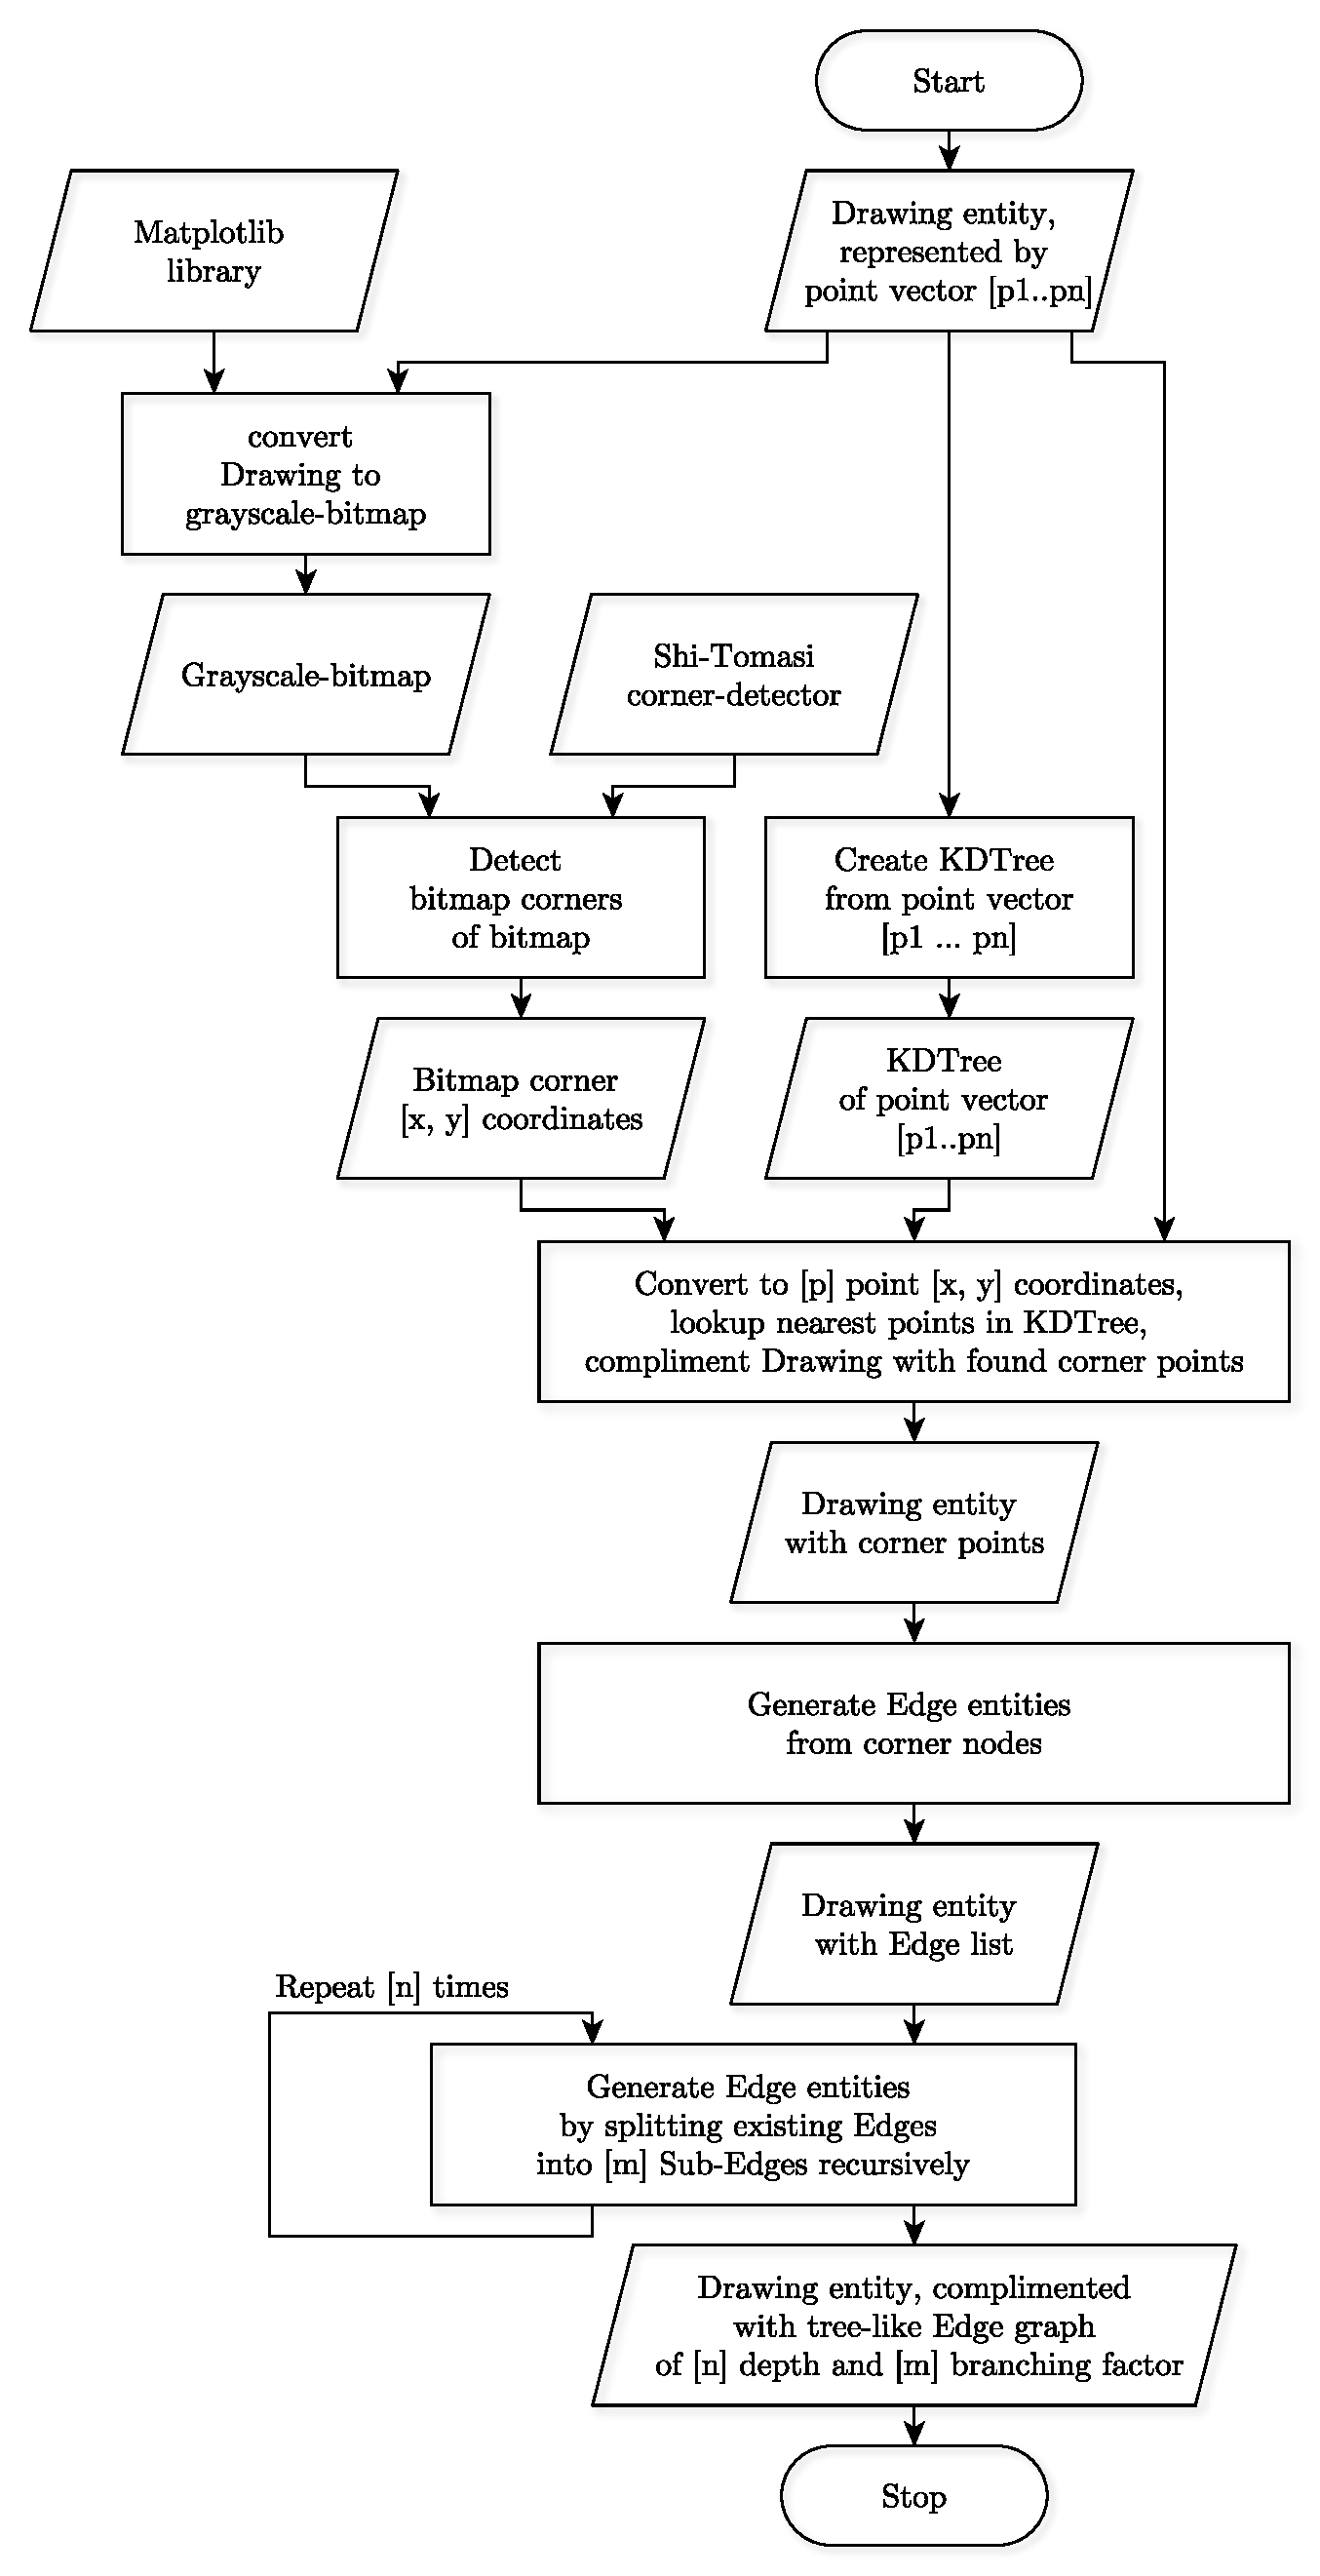
\includegraphics[width=0.75\textwidth]
        {images/clustering/flow-clustering}
    \caption{Clustering of the \textit{Drawing} entity --- Flow Diagram}
    \label{flow-clustering}
\end{figure}
